% !TEX program = pdflatex
\PassOptionsToPackage{backref=page}{hyperref}
\documentclass[9pt, aspectratio=169]{beamer}
% \usefonttheme[onlymath]{serif}

%%% === ADDITIONAL PACKAGES
\usepackage[T2A]{fontenc}
\usepackage[utf8]{inputenc}
\usepackage[russian]{babel}
\usepackage{animate}
\usepackage{caption}
\usepackage{subcaption}
\usepackage{tikz}
\usepackage{cancel}
\usepackage{booktabs}
\usepackage{ stmaryrd }
\usepackage[export]{adjustbox}
\usepackage{fontawesome5}
\usepackage{algorithmic}
\usepackage{yfonts}
\graphicspath{{../files/}}

% \LinesNumbered
\newcommand{\theHalgorithm}{\arabic{algorithm}}
\usepackage[ruled,vlined]{algorithm2e}
\renewcommand{\algorithmicrequire}{\textbf{Input:}}
\renewcommand{\algorithmicensure}{\textbf{Output:}}
\newcommand{\vect}[1]{\boldsymbol{\mathbf{#1}}}


%%% === TEMPLATE
\setbeamerfont{title}{series=\bfseries}
\setbeamerfont{frametitle}{series=\bfseries, size=\fontsize{12}{14}}

\setbeamersize
{
    text margin left=0.214cm,
    text margin right=0.214cm
}

\usefonttheme[onlymath]{serif}
\setbeamertemplate{bibliography item}{\insertbiblabel}
\setbeamertemplate{itemize items}[circle] % For level-1 itemize
\setbeamertemplate{itemize subitem}[circle] % For level-2 (subitems)
\setbeamertemplate{itemize subsubitem}[circle] % For level-3 (subsubitems)

\addtobeamertemplate{footline}{\raisebox{-1.3pt}{\href{https://fmin.xyz}{
\includegraphics[width=1cm]{logo.pdf}}} \hspace{0.2cm} \hbox{\insertsection \hspace{0.2cm} | \hspace{0.2cm}\insertsubsection} \hfill \href{https://hse24.fmin.xyz}{\faGem[regular]} \hspace{0.04cm} \href{https://github.com/MerkulovDaniil/hse24}{\faGithub} \hspace{0.07cm} \href{https://t.me/fminxyz}{\faTelegram} \hspace{0.4cm}\hbox{\insertframenumber \hspace{0.1cm}}
  \vskip0pt
}

\usenavigationsymbolstemplate{}

%%% === ADDITIONAL COMMANDS
\newcommand*{\Scale}[2][4]{\scalebox{#1}{$#2$}}%
\newcommand{\argmin}{\operatornamewithlimits{argmin}}
\newcommand{\argmax}{\operatornamewithlimits{argmax}}
\newcommand{\la}{\langle}
\newcommand{\ra}{\rangle}

\title{Описание курса}
\author{Даня Меркулов}
\date{}

\begin{document}
 \begin{frame}
  \begin{minipage}{0.618\textwidth}
    \centering{\Large \bfseries Методы Оптимизации в Машинном Обучении}\\
    \vspace{5pt}
    \centering{Факультет Компьютерных Наук\\ ВШЭ}\\
    \vspace{10pt}
    
\includegraphics[width=\textwidth]{back.png}
  \end{minipage}%
  \begin{minipage}{0.382\textwidth}
    \maketitle
  \end{minipage}
 \end{frame}

% \thispagestyle{empty}
% \begin{frame}{Outline}
%   \tableofcontents
% \end{frame}

\section{Структура курса}
\begin{frame}{Общая информация о курсе}
\begin{minipage}{0.618\textwidth}
    \begin{itemize}
        \item Лектор - Меркулов Даниил Максимович (Сколтех, МФТИ, ВШЭ)
        \item Курс для студентов 3 курса ПМИ ФКН ВШЭ. 1 лекция + 1 семинар в неделю.
        \item Старт учебной недели - 8 января. Длительность 20 недель.
        \item Курс охватывает темы выпуклой, невыпуклой, непрерывной  оптимизации, особенно мотивированные задачами и приложениями в Машинном Обучении. Рассматриваются разные темы - от фундаментальных материалов до недавних исследований.
    \end{itemize}
  \end{minipage}%
  \begin{minipage}{0.382\textwidth}
    \centering{
        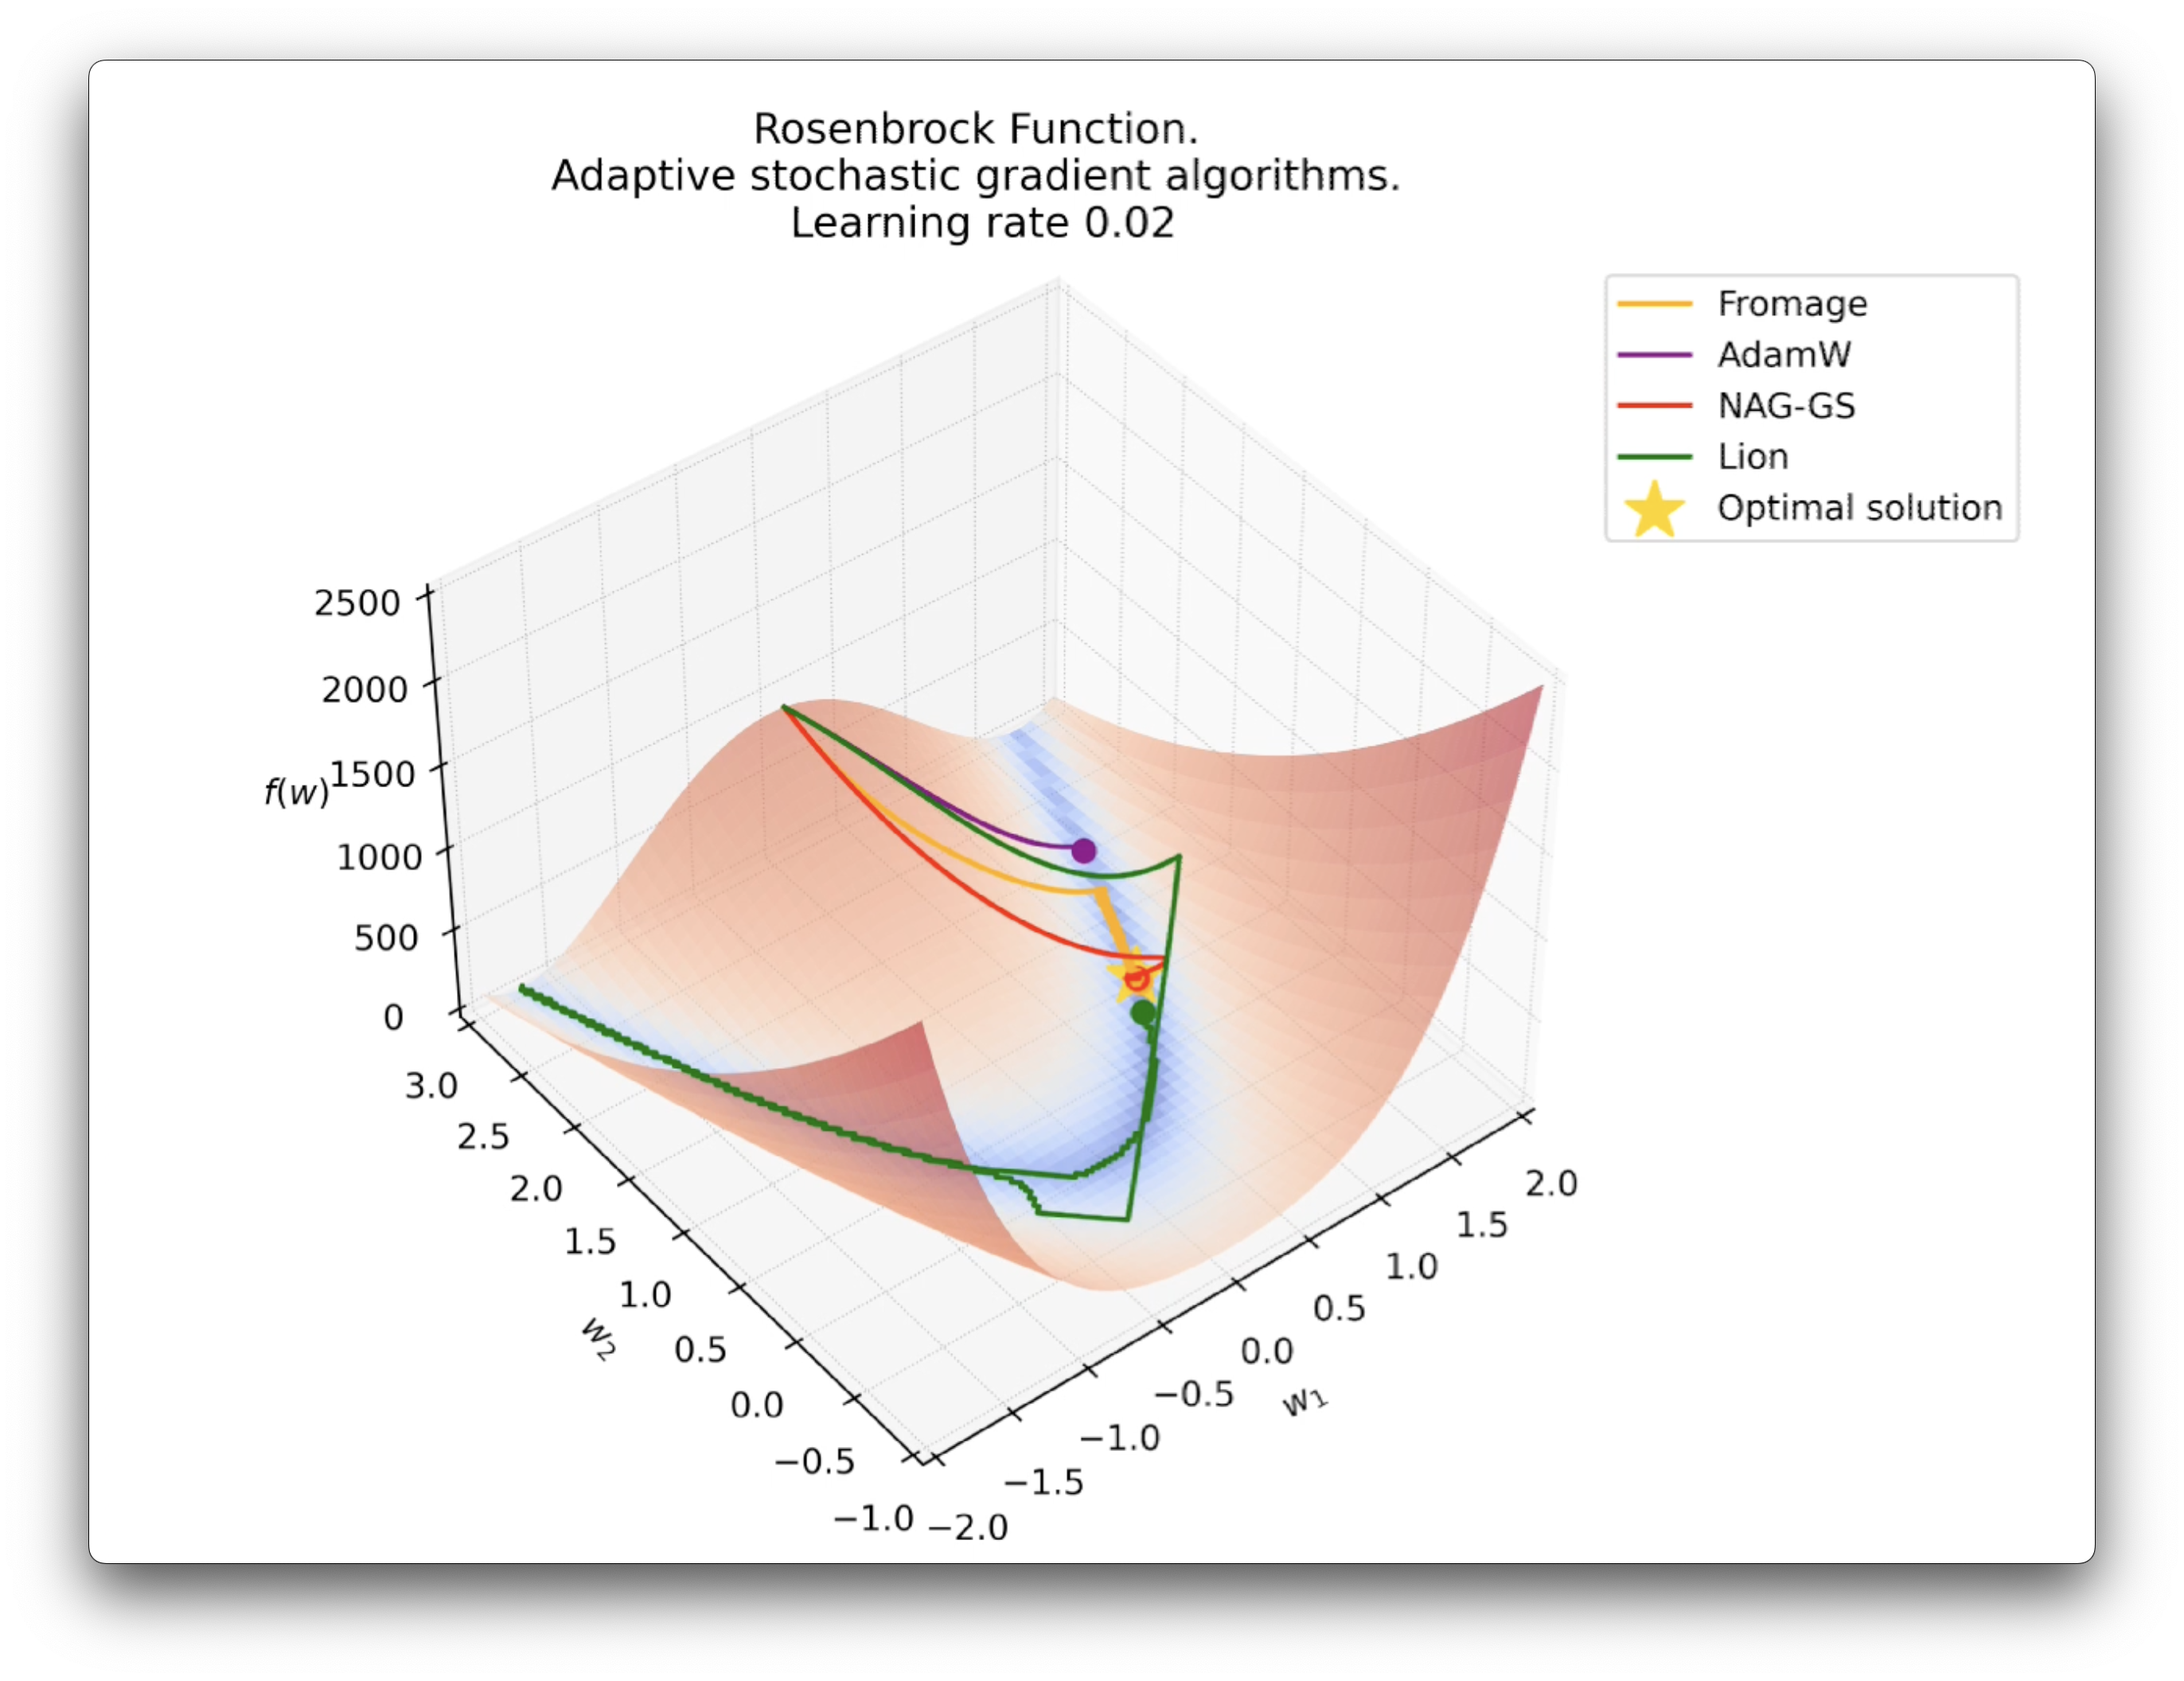
\includegraphics[width=.9\linewidth]{sgd.png}
    }
  \end{minipage}
\end{frame}

\subsection{Темы лекций (программа и количество лекций могут быть немного изменены)}

\begin{frame}{I. База 1}
    \begin{minipage}{0.618\textwidth}
        \begin{enumerate}
            \item Вспоминаем линейную алгебру. Некоторые матричные разложения. Скорость сходимости. Одномерная оптимизация. Неточная одномерная оптимизация.
            \item Градиент. Гессиан. Матрично-векторное дифференцирование. Автоматическое дифференцирование. Вычислительный граф.
            \item Выпуклость. Выпуклые множества. Выпуклые функциии. Неравенство Йенсена. Сильно выпулые функции. Условие Поляка - Лоясиевича.
        \end{enumerate}
      \end{minipage}%
      \begin{minipage}{0.382\textwidth}
        \centering{
        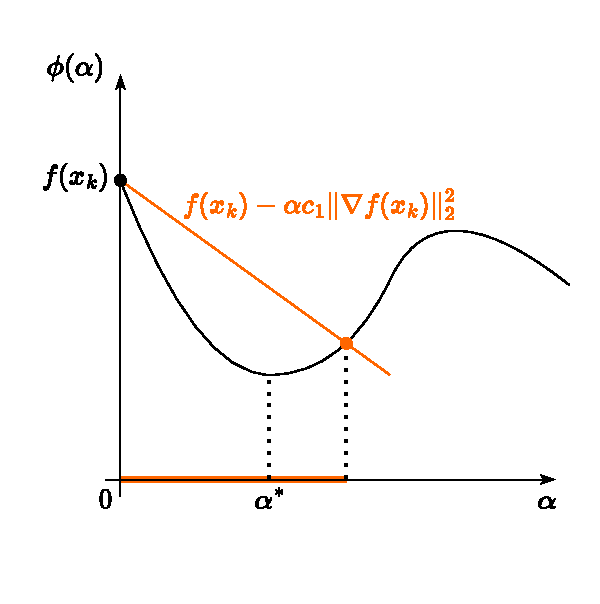
\includegraphics[width=\linewidth]{ls.pdf}
    }
      \end{minipage}
\end{frame}

\begin{frame}{II. База 2}
    \begin{minipage}{0.618\textwidth}
        \begin{enumerate}
            \setcounter{enumi}{3}
            \item Условия оптимальности. Функция Лагранжа. Множители Лагранжа. Теорема Каруша - Куна - Таккера.
            \item Двойственность. Введение в двойственность. Двойственная задача. Анализ чувствительности.
            \item Задача линейного программирования. Симплекс метод.
        \end{enumerate}
      \end{minipage}%
      \begin{minipage}{0.382\textwidth}
        \centering{
        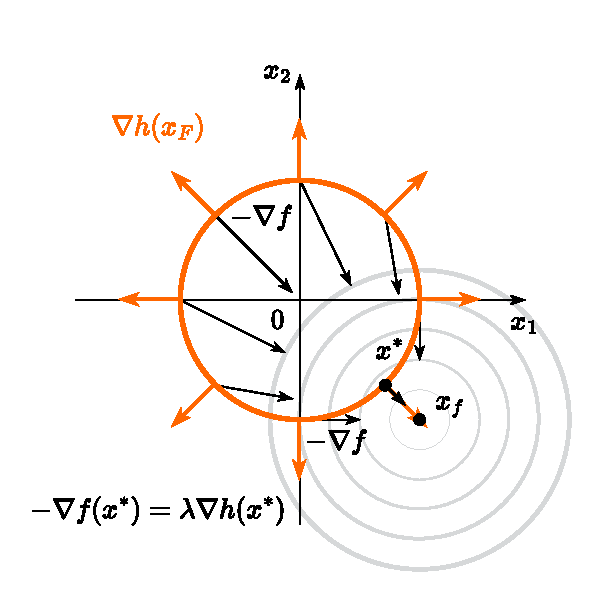
\includegraphics[width=\linewidth]{kkt.pdf}
    }
      \end{minipage}
\end{frame}

\begin{frame}{III. Методы первого порядка}
    \begin{minipage}{0.618\textwidth}
        \begin{enumerate}
            \setcounter{enumi}{6}
            \item Градиентный спуск. Теоремы сходимости в гладком случае (выпуклые, сильно выпуклые, PL). Верхние и нижние оценки сходимости.
            \item Ускоренные градиентные методы. Метод Поляка, Нестерова.
            \item Субградиент. Субдифференциал. Субградиентный спуск. Теоремы сходимости в негладком случае. Особенности работы градиентного метода в практических негладких задачах.
        \end{enumerate}
      \end{minipage}%
      \begin{minipage}{0.382\textwidth}
        \centering{
        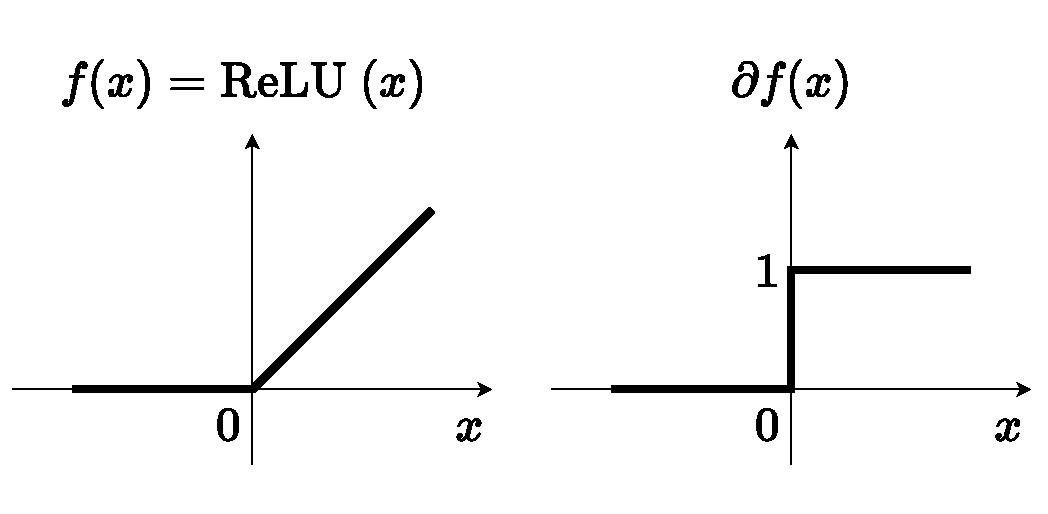
\includegraphics[width=\linewidth]{subgrad.pdf}
    }
      \end{minipage}
\end{frame}

\begin{frame}{IV. Ускорения, ограничения, более высокие порядки}
    \begin{minipage}{0.618\textwidth}
        \begin{enumerate}
            \setcounter{enumi}{9}
            \item Проксимальный градиентный метод. Метод Франк-Вульфа. Метод проекции градиента. 
            \item Метод сопряженных градиентов.
            \item Метод натурального градиента. K-FAC. Идея метода зеркального спуска. 
            \item Метод Ньютона. Квазиньютоновские методы.
            \item Введение в методы внутренней точки.
        \end{enumerate}
      \end{minipage}%
      \begin{minipage}{0.382\textwidth}
        \centering{
        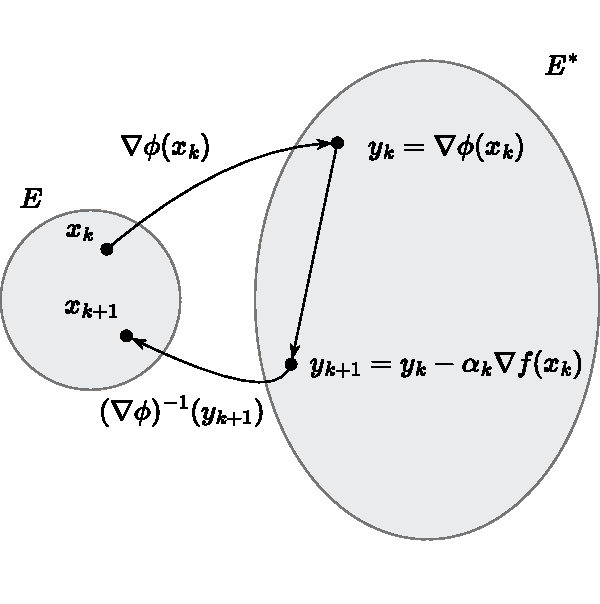
\includegraphics[width=\linewidth]{MD.pdf}
    }
      \end{minipage}
\end{frame}

\begin{frame}{V. Оптимизация в нейронных сетях и недавние исследования}
    \begin{minipage}{0.618\textwidth}
        \begin{enumerate}
            \setcounter{enumi}{14}
            \item Стохастический градиентный спуск. Адаптивные стохастические градиентные алгоритмы: AdaDelta, RMSProp, Adam, Nadam.
            \item Методы редукции дисперсии: SAG, SVRG, SAGA.
            \item Градиентный поток и диффузия. Методы оптимизации в непрерывном времени.
            \item Седловые задачи. Минимакс. Обучение GAN.
            \item Обобщающая способность моделей машинного обучения. Neural Tangent Kernel. Mode connectivity.
            \item Инициализация. Регуляризация. Residual connections. Вопросы обучения больших моделей. Lars, Lamb. Расписания learning rate. Warm-up. Клиппинг.
        \end{enumerate}
      \end{minipage}%
      \begin{minipage}{0.382\textwidth}
        \begin{figure}
            \centering
            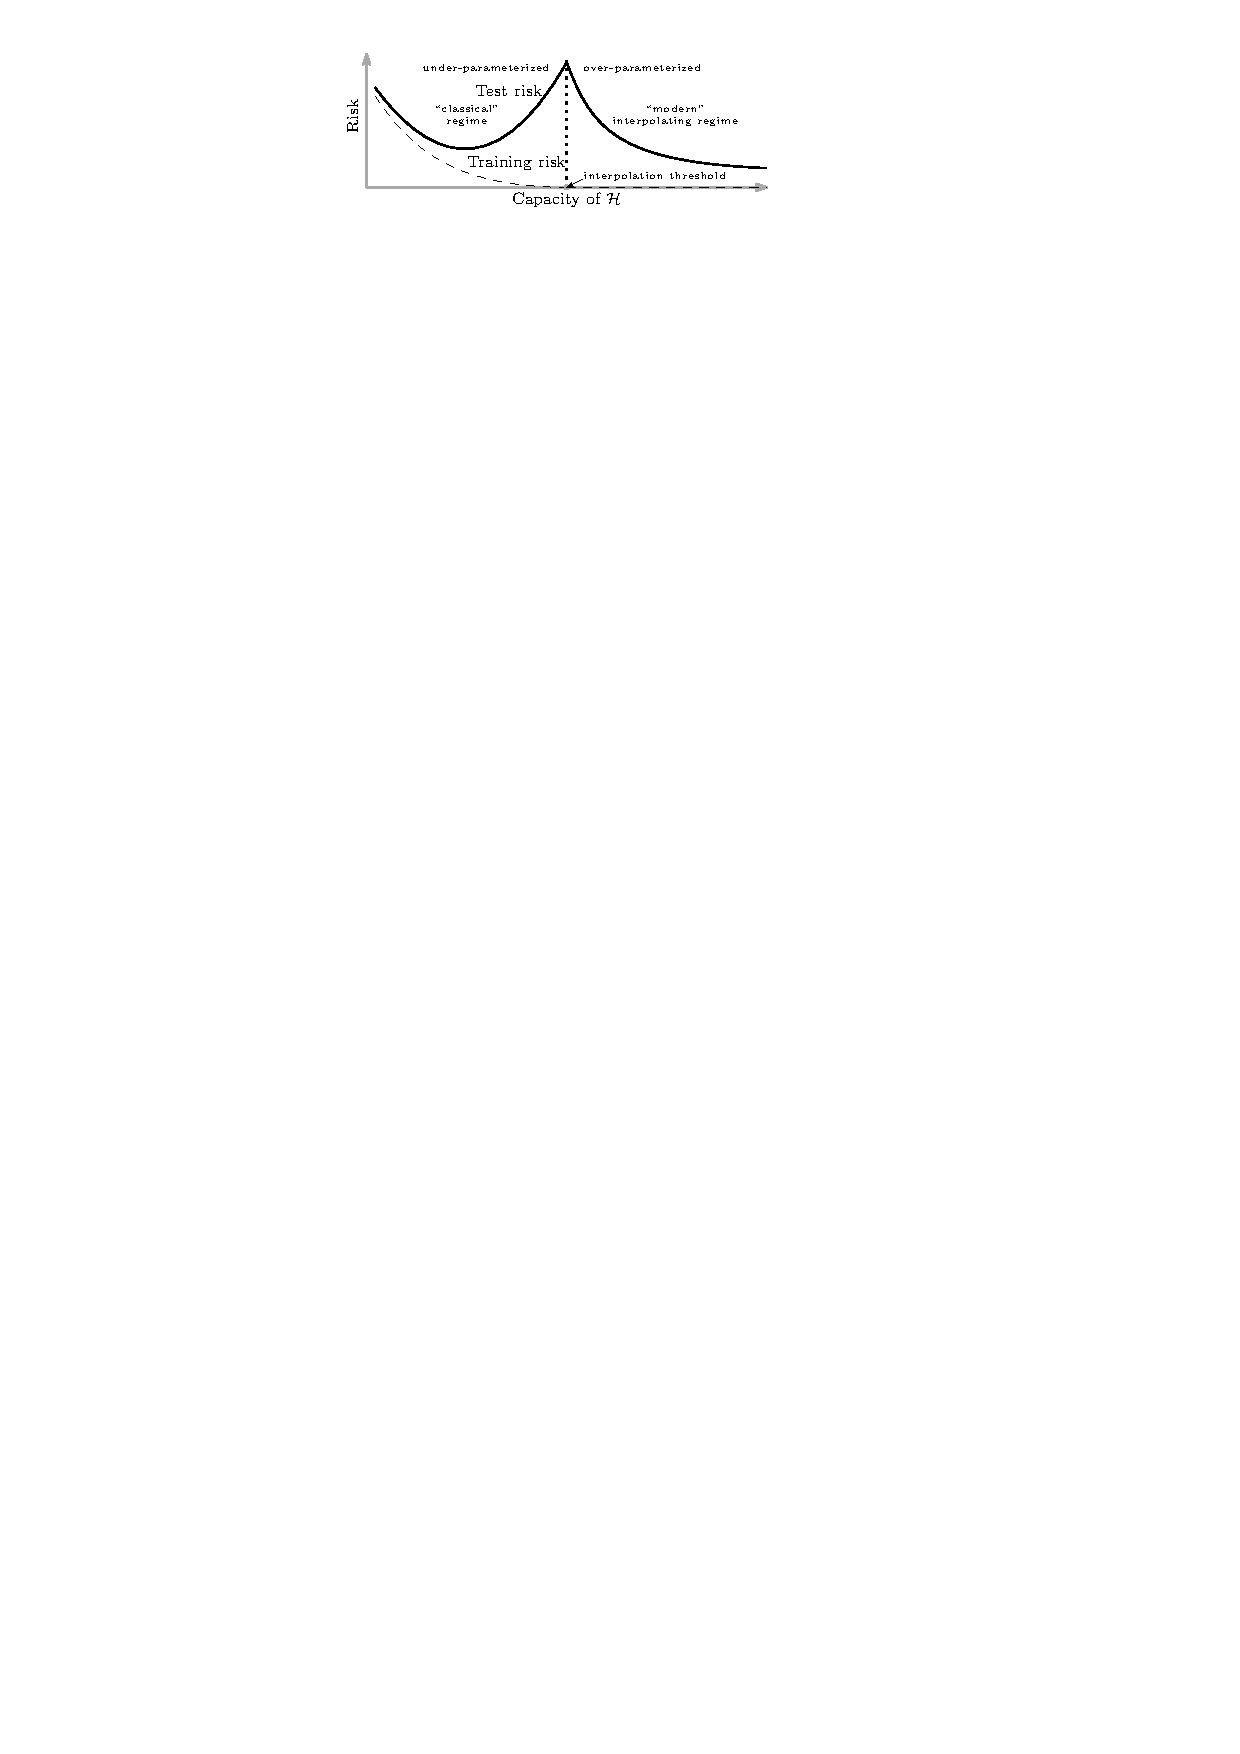
\includegraphics[width=\linewidth]{doubledescent}
            \caption{Source: \cite{belkin2019reconciling}}
        \end{figure}
        \centering
        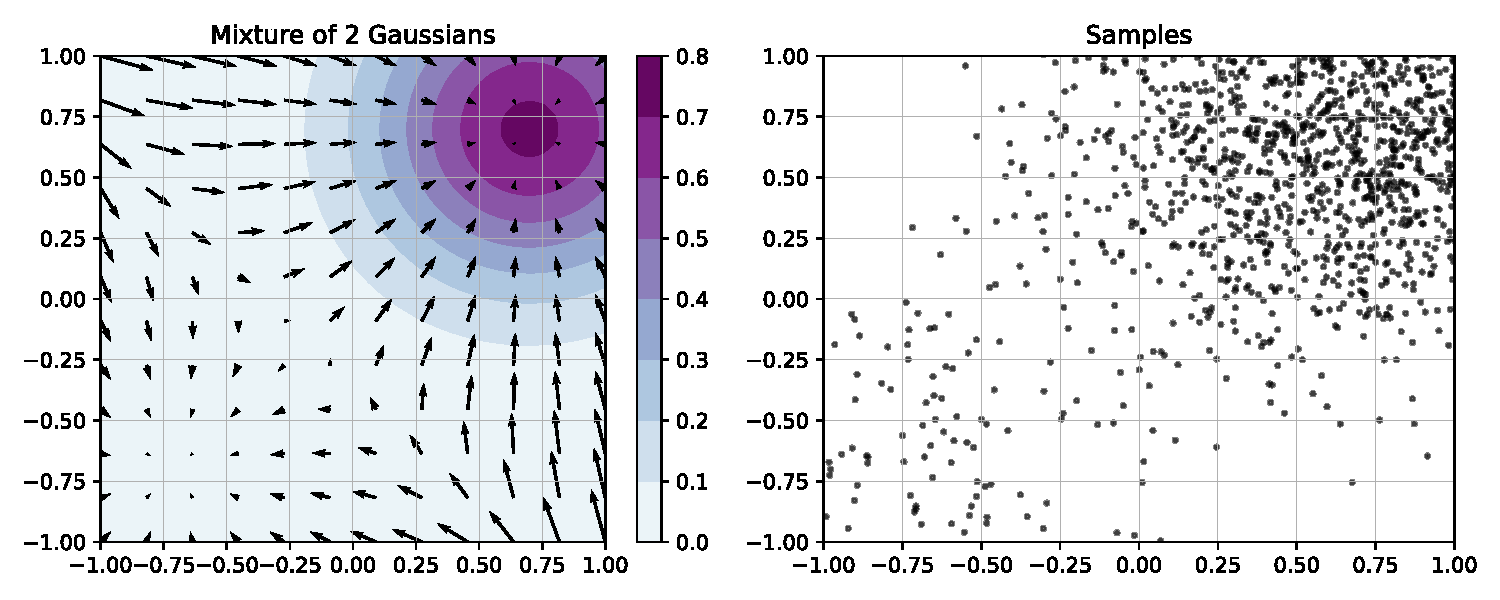
\includegraphics[width=\linewidth]{diff.pdf}
    \end{minipage}
\end{frame}

\section{Оценивание}
\begin{frame}{Оценивание}
    Оценка за курс вычисляется по следующей формуле:

    $$
    \text{grade} = \text{round}\left(\min\left(10, \begin{bmatrix}
        0.15 \\ 0.35 \\ 0.25 \\ 0.25
    \end{bmatrix}^T \begin{bmatrix}
        \text{Test} \\ \text{HW} \\ \text{Colloquium} \\ \text{Exam}
    \end{bmatrix} + 0.5\min \left(1, \dfrac{\text{\faGithub}}{10}\right)+ 0.5 \text{ \faPaw}\right)\right)
    $$

    \begin{itemize}
        \item Test, HW, Colloquium, Exam - оценки за соответствующие активности от $0$ до $10$.
        \item Тесты проводятся (по возможности) на каждой лекции по материалам предыдущей лекции. За пропущенный по неуважительной причине тест ставится $0$. 
        \item Оценки за тесты и коллоквиум являются блокирующими (если набрать меньше $3.5$ из $10$, то курс не сдан). 
        \item Домашние работы выдаются по темам каждого занятия в конце лекции.
        \item \faGithub~- количество принятых коммитов в \underline{\href{https://github.com/MerkulovDaniil/optim}{главный репозиторий}} с учебными материалами.
        \item \faPaw \; $=1$, если пропущены менее 25\% семинаров не по уважительной причине. Иначе \faPaw \;$=0$.
    \end{itemize}
    
\end{frame}

\begin{frame}{Коллоквиум}
    \begin{itemize}
        \item Коллоквиум пройдёт в конце учебного года (точная дата будет объявлена позднее) и будет включать в себя только материалы по темам прошедших лекций.
        \item Оценка за коллоквиум складывается из 4 частей
        \begin{itemize}
            \item Вопросы по формулировкам - 2 балла
            \item Теорема с доказательством - 3 балла
            \item Решение задачи - 3 балла
            \item Дополнительный вопрос - 2 балла
        \end{itemize}
        \item Сначала выдаются 4 случайных определения/формулировки из списка. На подготовку дается 10 минут. При правильном ответе хотя бы на 3 из 4 определений/формулировок коллоквиум продолжается дальше, и вы получаете $x-2$ баллов, где $x$ – число верно отвеченных вопросов. В противном случае за коллоквиум выставляется 0 баллов.
        \item При успешной сдаче определений вам выдается билет, содержащий теоретический вопрос на доказательство, а также задачу. На подготовку к ответу дается 40 минут. Теоретический вопрос на доказательства будет по теоремам из списка. Для подготовки к задачам советуем повторить домашние задания, а также задачи с семинаров.
        В процессе беседы по предыдущим пунктам экзаменатор может задавать уточняющие вопросы. 
        \item После ответа на предыдущие этапы экзаменатор задает дополнительный вопрос, например, задачу или вопрос, связанный с теорией. Ответ на дополнительный вопрос оценивается в 2 балла.
    \end{itemize}
\end{frame}

\begin{frame}{Экзамен}
    \begin{itemize}
        \item Письменный экзамен проводится в конце учебного года и сожержит в себе практические и теоретические вопросы по всем темам, которые обсуждали на лекциях и семинарах.
        \item На экзамене нельзя пользоваться справочными материалами. При себе необходимо иметь только ручку для написания экзамена.
    \end{itemize}
\end{frame}

\section{Материалы}

\begin{frame}{Материалы}
    Книги:
    \begin{itemize}
        \item Boyd S. P., Vandenberghe L. Convex optimization. – Cambridge university press, 2004.
        \item Nocedal J., Wright S. J. (ed.). Numerical optimization. – New York, NY : Springer New York, 1999.
        \item Nesterov Y. et al. Lectures on convex optimization. – Berlin : Springer, 2018. – Т. 137. – С. 576.
        \item Жадан В. Г. Методы оптимизации. Части 1, 2, 3 //М.: МФТИ. – 2014.
    \end{itemize}

    Ссылки

    \bibliographystyle{plain} % or another style like alpha, abbrv, etc.
    \bibliography{biblio} 

\end{frame}

\end{document}